\begin{center}
\textsc{\Large Laboratorio 12}~\\
{\large Vídeo Juegos, Diseño, Programación}~\\
\emph{Animaciones}
\end{center}

\section{Pre-Laboratorio}
\todo[inline]{Por hacer.}

\section{Introducción}
\setlength\intextsep{0pt}
\begin{wrapfigure}[8]{r}{0.2\linewidth}
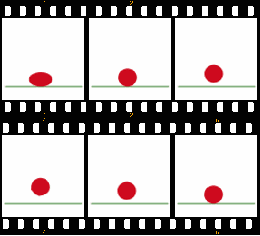
\includegraphics[width=\linewidth]{semana12/anim_frames.png}
\caption{Cuadros de animación de una pelota rebotando.}
\label{fig:particles}
\end{wrapfigure}
Animación es el proceso de crear la apariencia de movimiento y cambios de forma mostrando rápidamente una secuencia de imágenes estáticas que difieren muy poco entre unas y otras. Los animadores son artistas que se especializan en la creación de animación.

La mayoría de los juegos modernos tienen algún objeto o personaje que necesita ser animado. La excepción en esto esta en juegos de carreras, simuladores o puzzles (e incluso en estos algunos detalles podrían estar animados) \cite[p.~381]{erikgamedevelopment}.
\section{Actividad}
\todo[inline]{Por hacer.}